% \pagestyle{empty}
\chapter{Introduction}

Scene understanding, tracking of moving objects, and moving object anticipation are key aspects in the area of Computer Vision. Anticipation of moving objects is an actively researched problem across domains such as robotics, autonomous vehicles, augmented reality, and surveillance.

In an autonomous driving setting, identifying both vehicle and pedestrian intent and predicting the next position helps in taking appropriate actions to avert collision. It is also important in order to maintain safe distances from moving objects. It also enables rational decision-making with respect to all objects in the surrounding area. Even at slow driving speeds of 30 to 40 km per hour, anticipating positions in the next 1 to 2 seconds are useful in making safe driving decisions. Pedestrian path prediction is currently used Advanced Driver Assisted Systems (ADAS) to alert drivers of Vulnerable Road Users (VRUs).

Pedestrian path prediction is a highly challenging area as it is dependent on the behaviour of pedestrians, and pedestrian movement can be highly difficult to predict due to the highly dynamic nature of humans. People may start walking, stop or start running abruptly, and these actions might not be predictable based only on visual clues. 
However, with  improved understanding of context, and feeding details of the surrounding environment, it is envisioned to have a better understanding of human movement in a traffic setting. This would mean creation of a lot of hand-crafted inputs as features. However, with the advent of deep learning, it is hoped that the step of feature engineering can be skipped, so that the algorithm auto-detects features. This work aims at producing a deep learning model to predict pedestrian trajectory, panning out to in the future to be able to incorporate multiple useful data sources. 

Path and trajectory are used interchangeably and mean the same in this work.

\section{Objective}

To predict pedestrian's future trajectory based on cues and information from the current frames. 

\section{Outline}
This dissertation is structured in the following manner. Chapter 1 gives a brief introduction of the problem we are trying to solve and its relevance today. It also gives a background of Deep Learning, so that the reader is familiar with the technique to be adopted in this work. Chapter 2 presents a review of the works related to this problem. Chapter 3 states the problem specifically w.r.t the dataset, and establishes evaluation metrics that will be used for defining the success of the experiment. Chapter 4 details the experimental setup and the describes the dataset to be used. Chapter 5 details the results of the experiments and discussion.

% Write this portion after completion. Should give an overview of this document from this point. refer %https://www.ias.informatik.tu-darmstadt.de/uploads/Theses/HajiGhasemi_MScThesis_2013.pdf





\section{Deep Learning}
\subsection{Background and History}
Deep learning is a field that came into being with the idea of understanding how the human brain learns information and be able to extend that to computers.
The first implemented work in the field of deep learning was in the work of \citet{ivakhnenko_cybernetic_1973}.
Deep learning is a data intensive task, and performs better on very large datasets, and expensive computation. Among the first applications of Deep Learning, recognition of handwritten zipcodes done by Yann LeCunn in 1989 in \cite{lecun_backpropagation_1989} is most popular. While the algorithm worked, it took 3 days for training the algorithm.
With the increase of more computationally powerful machines, more and more experiments with Deep Learning were performed, and now Deep Learning is a part of many state-of-the-art applications, across different domains\cite{sak_fast_2015}\cite{deng_deep_2013}\cite{li_constructing_2014}. Deep Learning rose to popularity in the years following 2011-2012, with its employment in the field of computer vision for object detection. In October 2012, a paper by Ciresan et al, demonstrated in the leading CVPR (Computer Vision and Pattern Recognition) conference  how incorporating max-pooling into Convolutional Neural Networks (CNNs) could break multiple benchmarks, and this saw the rise in popularity of Deep learning in research work. Following this, CNNs were successfully used in different image recognition challenges such as the ImageNet\cite{deng_imagenet:_2009}, Pascal VOC\cite{everingham_pascal_2010} and COCO\cite{lin_microsoft_2014} Challenges.

\subsection{Neural Networks}
Deep learning is a subset of Machine Learning, where neural networks are used. 
A simplistic view of Deep Learning algorithm is to consider it as an optimisation of certain parameters with respect to some constraints. The constraints are called losses or costs in the Deep Learning setup. The optimum value of the parameter is that value that minimises cost. Let's consider a situation where we are given an input variable \(x, \) and target variable y. The goal of the Deep Learning algorithm is to find a mapping \(f^*\), taking in \(x, \) and some parameters \((W, b)\), that correctly maps a given input variable \(x \) to the output \(y \), and gives the lowest value of Loss. The loss is the dissimilarity between the actual y, and the predicted output \(\hat{y}\), and is defined differently depending on the problem.

The difference between deep learning and other traditional machine learning applications is that the mapping that is to be learned, \( f^* \), may be a combination of multiple intermediate functions that are applied to intermediate inputs, and these are not explicitly defined by the programmer. The combination of different functions helps in building flexible decision-making algorithms. Here "flexible" means curved/ complicated decision boundary. The addition of multiple functions is done by having multiple layers with intermediate outputs. These layers is what lends deep learning its name. The presence of more layers makes a network deeper.
In a more formal specification of deep learning, is a complex representation of multi-level functions, modelled using neurons. A neuron is one operation performed on the input data. 


\begin{figure}
    \centering
    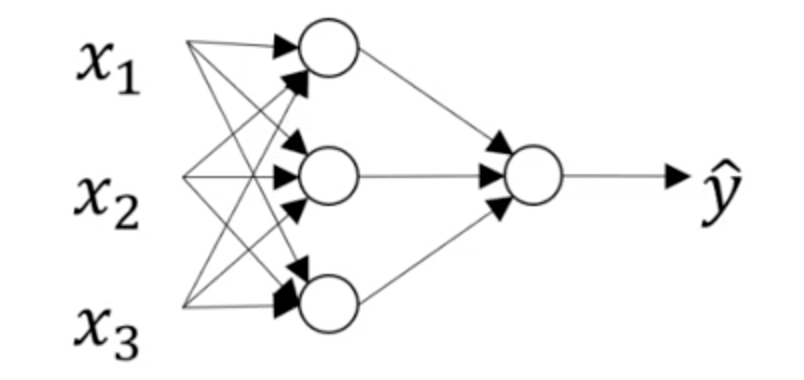
\includegraphics[height=0.15\paperheight]{Figures/nn_simple.png}
    \caption[A basic Neural Network diagram]{Simple Neural Network with 3 input variables predicting target variable y
    \cite{noauthor_neural_nodate}}
    \label{fig:NN_diagram}
\end{figure}

To give a more formal representation, we illustrate this by means of an example. We are given three input variables, and need to find the mapping to a variable, \(y\). Figure \ref{fig:NN_diagram} shows a neural network with 2 layers for this problem.  The number of layers is a tune-able parameter, and depends on the problem. Each layer has weights associated with it. These weights decide the relative importance to be given to each input at that layer. The problem is to find the optimum value of weights to be able to calculate a target variable as accurate as possible from the given input. It is represented by 2 equations:
\[z^{[1]}=W^{[1]}x+b^{[1]}\]
\[a^{[1]}=g(z^{[1]})\]
\[z^{[2]}=W^{[2]}x+b^{[2]}\]
\[a^{[2]}=g(z^{[2]})\]
where X is the matrix of inputs. W is a matrix of weights, and b is a bias vector. This can be vaguely equated to the linear regression equation \(y=mx + c\). The operations above are matrix multiplication and addition operations. Bias can be interpreted as the intercept in the linear regression equation. \(g\) is the called the activation function, and can be a any one of a \(sigmoid, tanh, reLU\) functions. \(a\) is called the activation - more specifically \(a^{[1]}\) is called the activation of the first layer. The activation of the last layer is the output of the neural network, and this is the calculated value of target, given the input. 

Thus, the parameters that need to be optimised are \(W\) and \(b\). There are various algorithms that can be employed to find the optimal value, the most common being back-propagation, a method of taking derivatives, and propagating the error through the network, and making adjustments to the parameters to arrive at the optimal value. Back-propagation is also known by the name of 'Gradient Descent'. The exact history of who invented it are unclear, however it can be seen as an extension of the famous Newton-Ralphson method. Recently, other variants of the algorithm such as ADAM\cite{kingma_adam:_2014}, RMSProp\cite{noauthor_neural_nodate-1} have been invented, and the choice of an optimisation algorithm is also an element of consideration while building and running Neural Networks. These optimisation algorithms have a parameter called learning rate, that decides how big each learning step needs to be. A value too large or too small will make the algorithm optimisation to take too much time to converge. Other techniques such as normalisation also help in the algorithm to converge faster. 


With a small dataset, deep learning only manages to perform rote learning of a data, and spit out outputs. Hence, when using small datasets, care must be taken to ensure that the algorithm does not do this, as otherwise the algorithm will fail on previously unseen data. This is called 'over-fitting'. In order to mitigate this effect, there are techniques called regularisation used.

The number of layers, number of nodes in a layer, normalisation, regularisation, learning rate are tune-able hyper-parameters in building Neural Networks.



Neural Networks also go by the name of Artifical Neural Networks (ANNs) and Multi-Layer Perceptrons (MLPs).

\subsection{Convolutional Neural Networks (CNNs)}
CNNs are specialised neural networks that are used for processing data that have grid-like topology. Convolutional networks are simply neural networks that use convolution in place of general matrix multiplication in at least one of their layers.

In computer vision problems, images are treated as grids of cells, each having some integer value. For example, in a black-and-white image, values in the cells could be 0 meaning black and 1 meaning white. Similarly, for grey-scale images, the integer value could be used for denoting intensity of brightness.

\begin{figure}
    \centering
    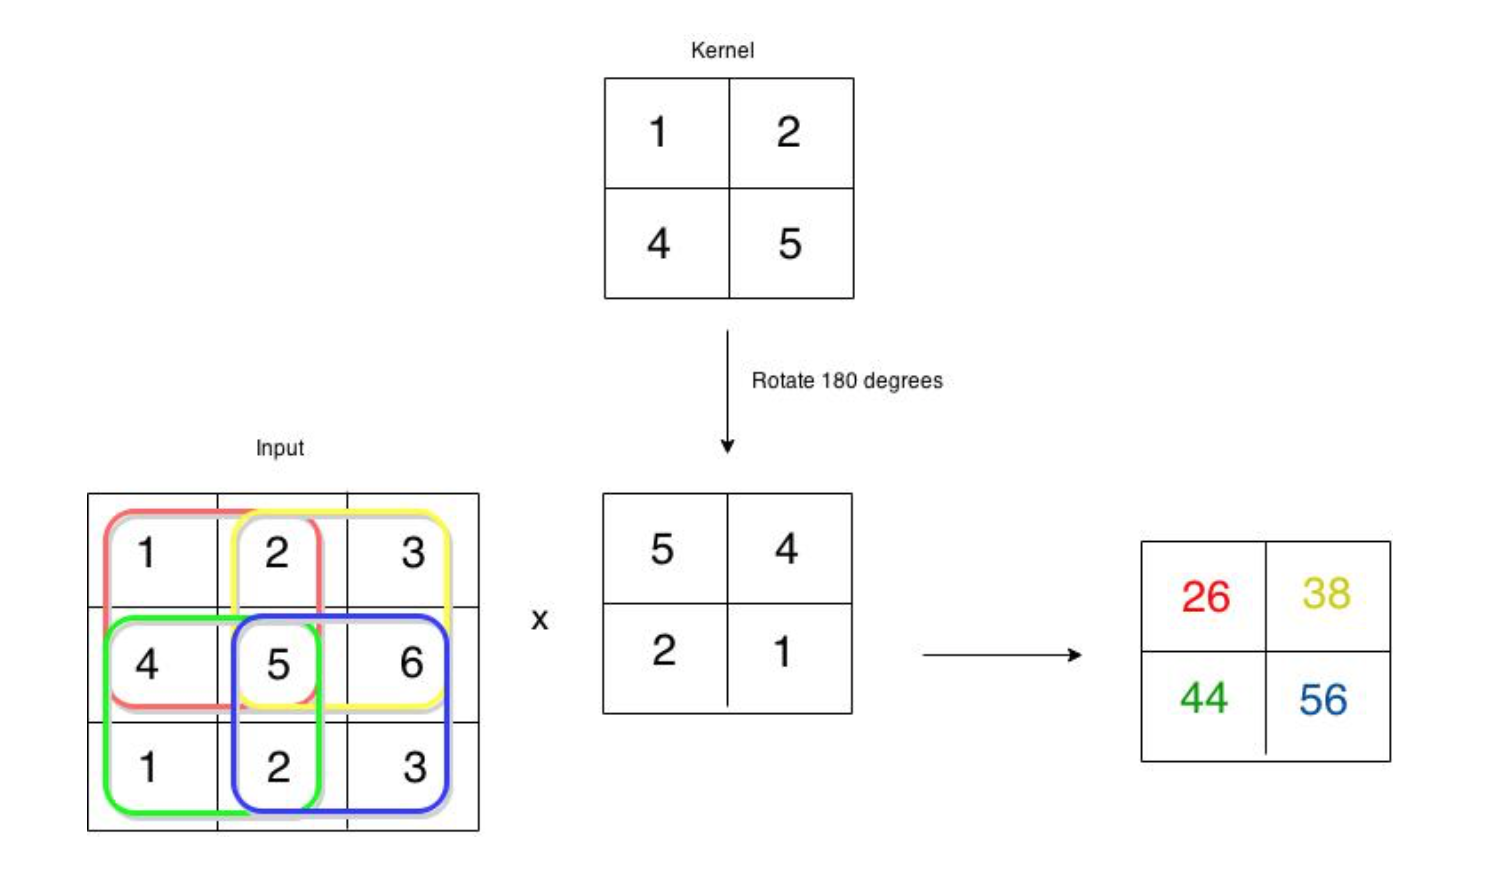
\includegraphics[height=0.2\paperheight]{Figures/CNN_explain.png}
    \caption[Convolution diagram]{Illustration of a convolution
    \cite{noauthor_convolutional_nodate}}
    \label{fig:convolution_diagram}
\end{figure}


A convolution is an operation applied to an image and can be used to identify, extract information or patterns from an image. Figure \ref{fig:convolution_diagram} shows a convolution operation. The \(3 * 3\)  grid is the input image, and the \(2 * 2\) grid is the filter/kernel/convolution - these terms mean the same, and refers to the parameters used to learn the features of the input image. The filter is moved across every \(2 * 2\) combination of boxes, and for each combination, each number is multiplied by the corresponding number on the box, and added up. When a filter is applied to an image it is called 'convolving' the image. Here for the first cell the value is computed as \( (5*1)+(4*2)+(4*2)+(5*1) = 26\).

Figure \ref{fig:convolution_edge_detection} is a simple example of a convolution for edge detection. 


\begin{figure}
    \centering
    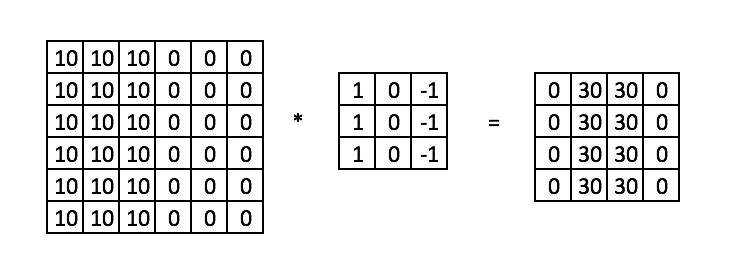
\includegraphics[height=0.15\paperheight]{Figures/cnn_edge_detection.png}
    \caption[Convolution for edge detection]{Convolution for edge detection}
    \label{fig:convolution_edge_detection}
\end{figure}
\subsection{Recurrent Neural Networks (RNNs)}

RNN stands for Recurrent Neural Network. 
RNNs were inspired to be built by the human nature of seeing patterns and being able to extrapolate from it. For example, when humans read a sentence, some words are not read with the same emphasis as others - there are key words that convey ideas.

Keeping this mind, an RNN is a modified version of a Neural Network that can take sequences as input, and learns a feature from all the intermediate inputs into it, and thus learns a sequence. In RNNs, there is parameter sharing across different parts of the sequence, as opposed to plain Neural Networks, and hence they are more suitable for sequential data. Figure \ref{fig:rnn_unit} shows an RNN. We can see from the diagram, there is information passed on from the previous point in the sequence, thus enabling flow of information from one part of the sequence to the next. This is just one RNN unit, and is equivalent to one node of the Neural network representation we have seen earlier. Thus, in addition to back-propagation through layers, there is an added extra functionality of back-propagation through time, within each node in each layer.

\begin{figure}
    \centering
    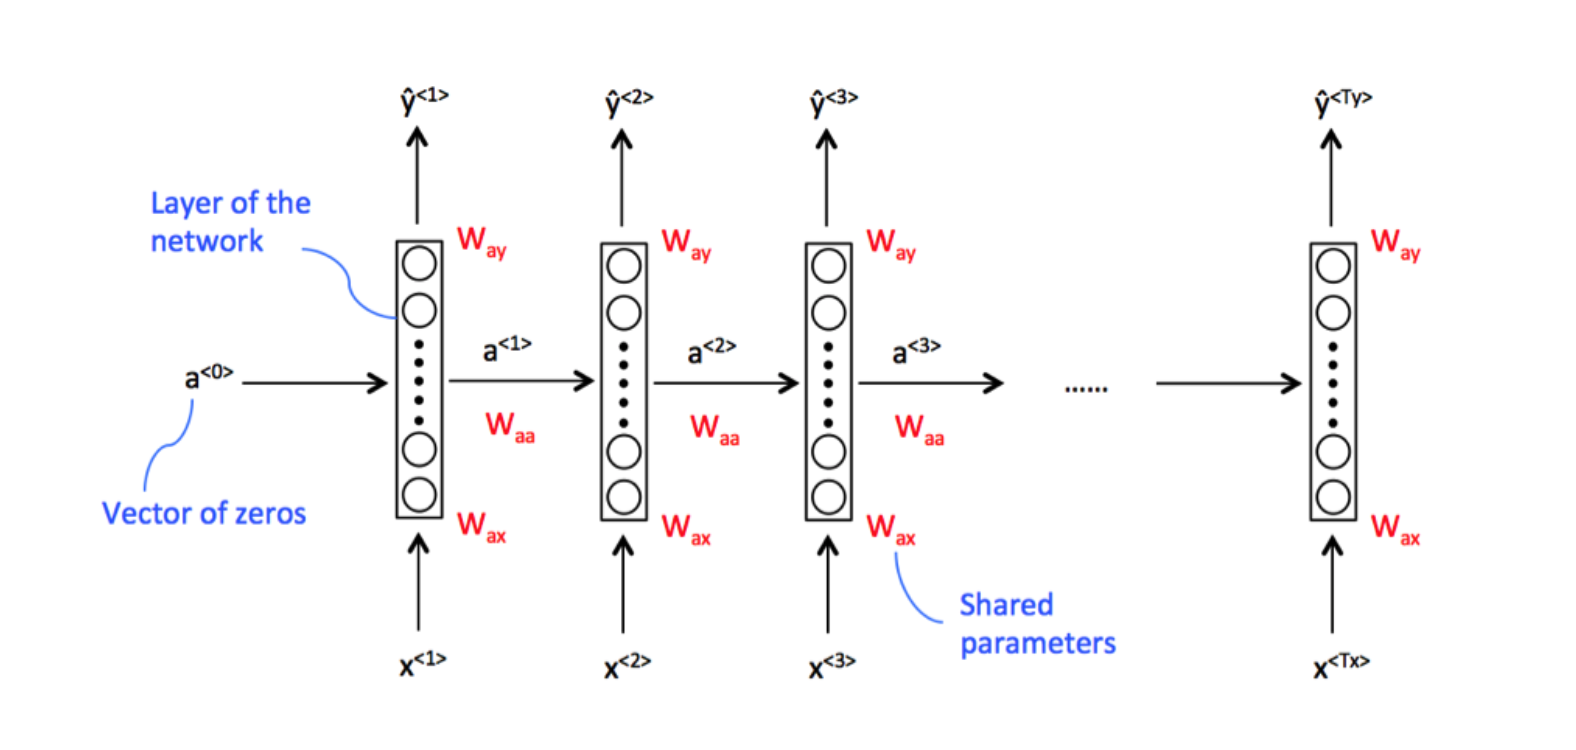
\includegraphics[height=0.2\paperheight]{Figures/rnn_simple.png}
    \caption[Structure of an RNN]{A layer in the RNN\cite{cavaioni_deeplearning_2018}}
    \label{fig:rnn_cell}
\end{figure}

\subsubsection{Simple RNN Unit}

\begin{figure}
    \centering
    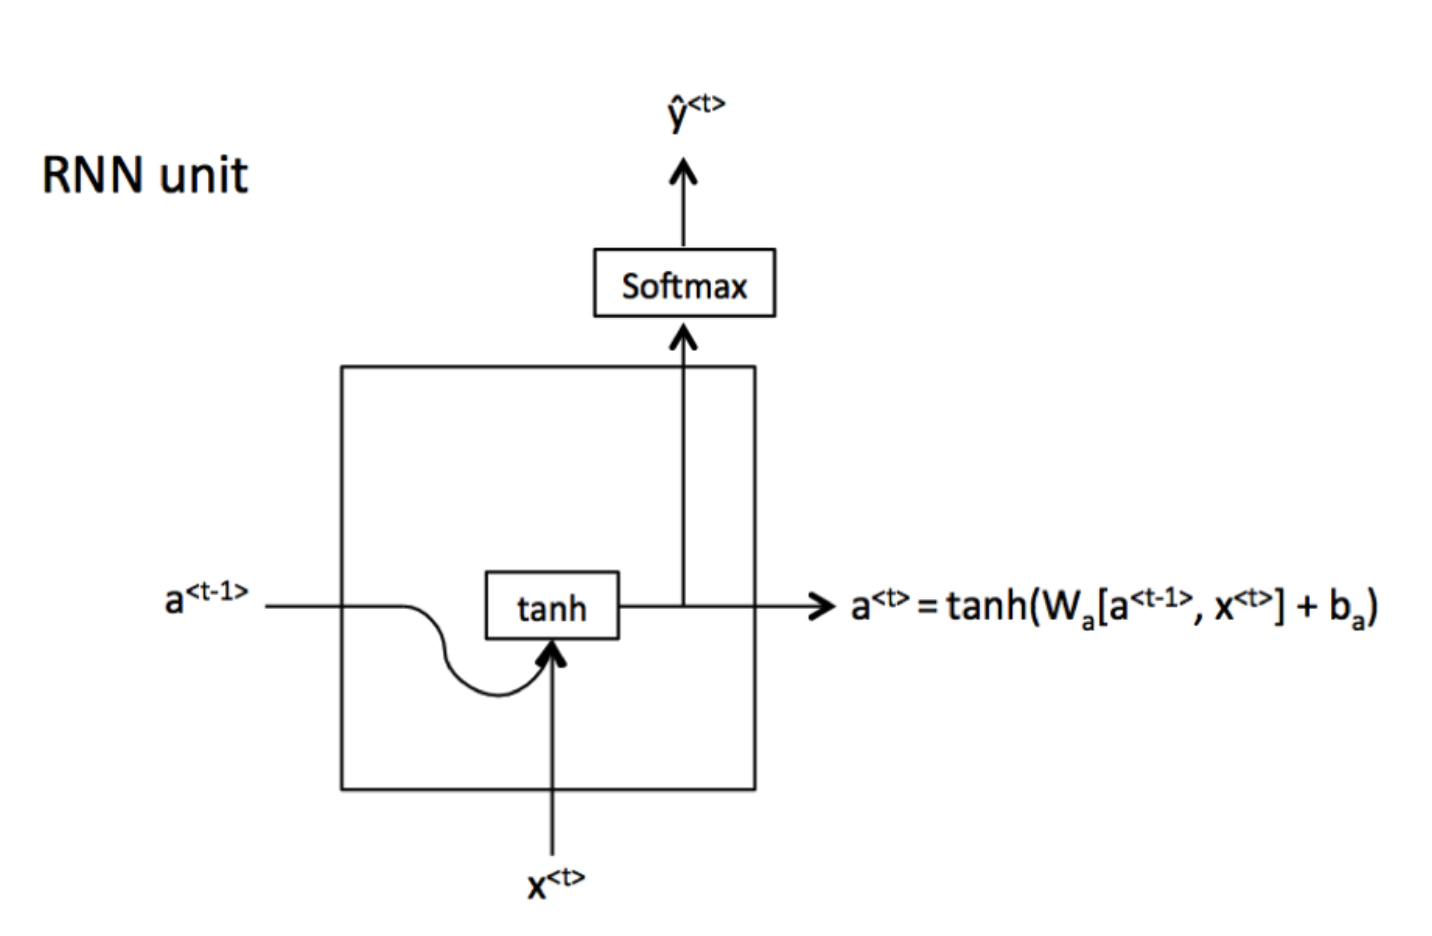
\includegraphics[height=0.2\paperheight]{Figures/RNN_unit.png}
    \caption[An RNN Unit]{RNN unit\cite{cavaioni_deeplearning_2018}}
    \label{fig:rnn_unit}
\end{figure}

In a formal representation of an RNN, the input is X of length \(T_x\). The input at the \(t^{th}\) point is represented by \(x^{<t>}\) and the corresponding output is \(y^{<t>}\). The activation is calculated as:\[a^{<t>}=g(W_{aa}a^{<t-1>}+W_{ax}X^{<t>}+b_a)\]
\(W_{ax}\) is a weight matrix multiplied by another matrix of type \(x\) (the second subscript), i.e., inputs, to get a matrix of the type \(a\) (the first subscript). We simplify the above equation as:
\[a^{<t>}=g_1(W_a[a^{t-1},x^{<t>}]+b)\]
In the above representation, the weight matrices \(W_{aa}\) and \(W_{ax}\) are combined by stacking each other, and similarly \(a^{<t-1>}\) and \(X^{<t>}\) are also stacked. The output is calculated as
\[\hat{y}^{<t>}=g_2(W_{ya}a^{<t>}+b_y)\]
Thus, the activation at every point is a combination of the activation from the previous time step, and of the input value of the current time step. This is how information is passed across time steps in an RNN.
Summarising, and simplifying the notations, we have the following equations that represent an RNN:
\[a^{<t>}=g_1(W_a[a^{t-1},x^{<t>}]+b)\]
\[\hat{y}^{<t>}=g_2(W_{y}a^{<t>}+b_y)\]

For a diagrammatic representation of these equations, refer \ref{fig:rnn_unit}. In this diagram, \(g_1\) is \(tanh\) and \(g_2\) is \(softmax\).




Due to this setup, where the error gradient has to back-propagate through multiple 'cells', it is difficult for the error to reach the initial nodes. This issue is called 'Vanishing gradient'. Due to this problem, the latter parts of the sequence have higher influence on the output when compared to the initial parts of the sequence. In order to counter these issues, modified RNN cells like Gated Recurrent Unit (GRU) and Long Short-Term Memory (LSTM) have been invented. We thus these in detail as this work uses a GRU cell.
\subsubsection{Gated Recurrent Unit (GRU)}
 \begin{figure}[h]
    \centering
    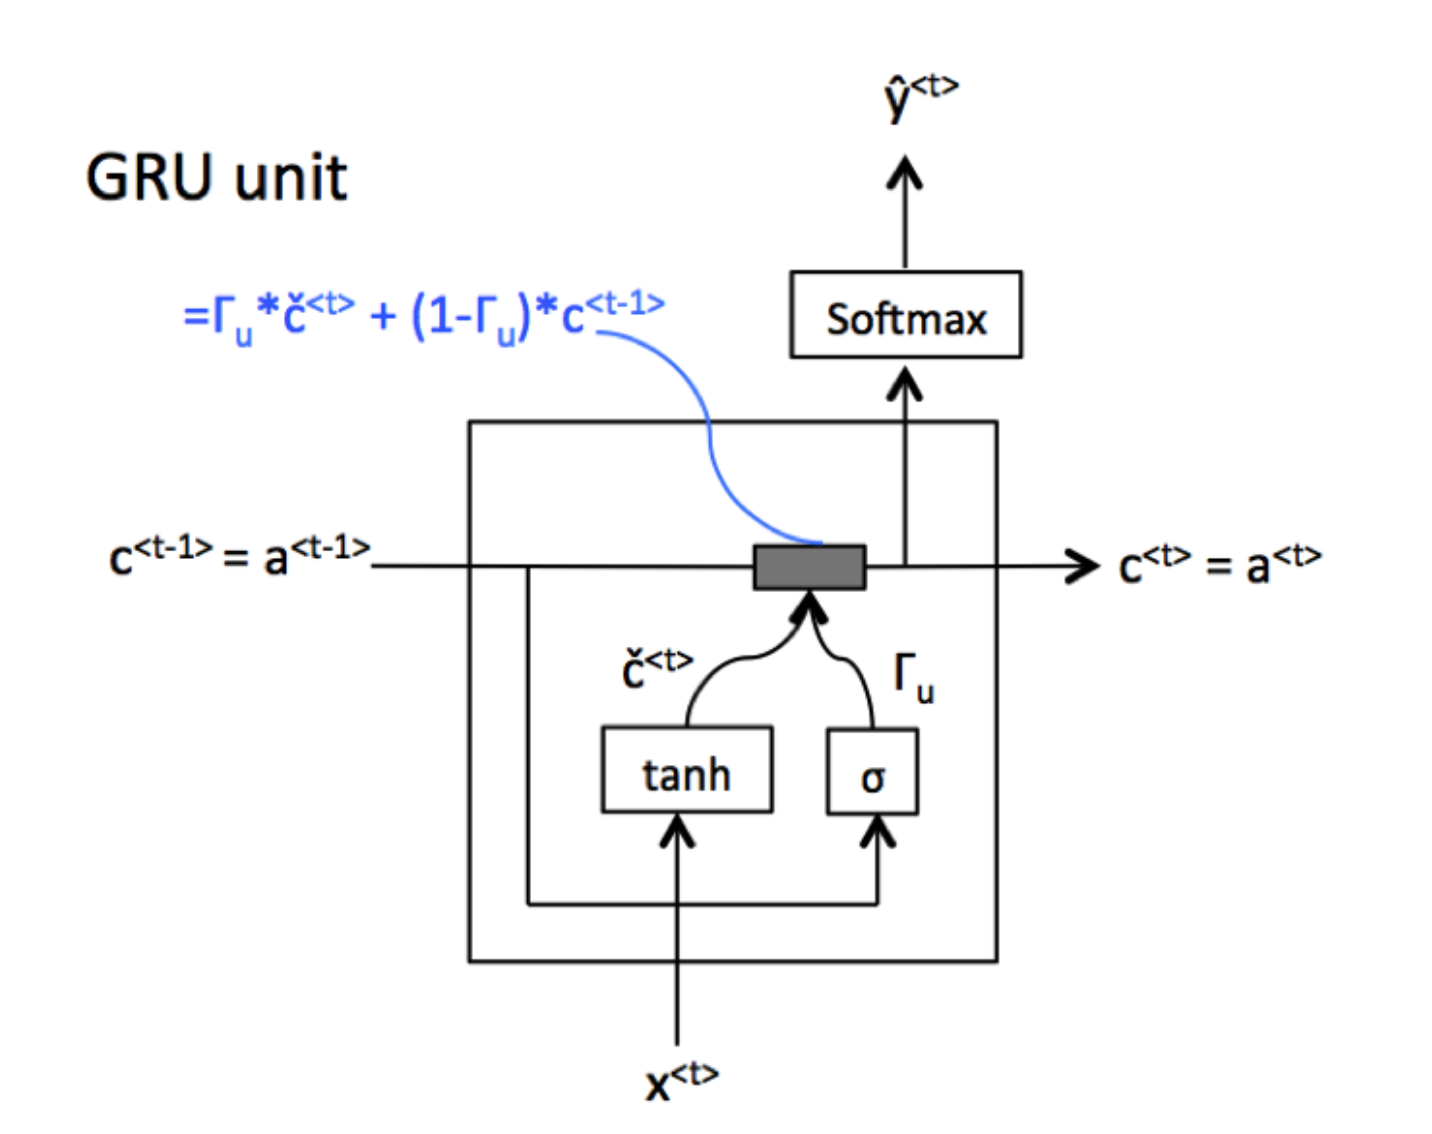
\includegraphics[height=0.25\paperheight]{Figures/GRU_cell.png}
    \caption[GRU Unit]{GRU unit\cite{cavaioni_deeplearning_2018}}
    \label{fig:gru_unit}
\end{figure}
GRUs were introduced in \cite{cho_properties_2014} and \cite{chung_empirical_2014}.
In GRUs, at each time step there is a memory state associated with it, called \(c^{<t>}\). It is initialised with the activation from the previous time step. At every time step, there is a candidate \(\Tilde{c}^{<t>}\) to replace \(c^{<t>}\). It is calculated using the following equation:
\[\Tilde{c}^{<t>}=tanh(W_c[\Gamma_r*c^{<t-1>},x^{<t>}]+b_c)\]
\(W_c\) and \(b\) are parameters. \(\Gamma_r\) is a relevance gate, used for deciding if \(c^{<t-1>}\) is relevant as the next candidate.\(\Gamma_r\) is calculated as:
\[\Gamma_r = \sigma(W_r[c^{<t-1>},x^{<t>}]+b_r)\]
In addition to this, there is an Update gate, \(\Gamma_u\) calculated as:
\[\Gamma_u = \sigma(W_u[c^{<t-1>},x^{<t>}]+b_u)\]
 \(\sigma\) represents the sigmoid function that converts inputs it gets into values between 0 and 1. Thus, the value of \(\Gamma_u\) ranges between 0 and 1. \(\Gamma_u\) decides if we should update the value of \(c^{<t>}\) or not. 
 
 The final update to the memory term at time \(t\) is performed using the following equation:
 \[c^{<t>}=\Gamma_u*\Tilde{c}^{<t>} + (1-\Gamma_u)*{c}^{<t-1>} \]
 Thus, the final value of the memory cell is decided by the update gate, with a certain weightage to the previous memory state, and some to the newly calculated candidate state. Figure \ref{fig:gru_unit} shows a diagrammatic representation of these equations.
 

\subsubsection{Long Short Term Memory (LSTM)}
LSTMs were introduced much before than GRUs, in \cite{hochreiter_long_1997}. LSTMs have a more complicated system of controls when compared to GRUs.
 \begin{figure}[h]
    \centering
    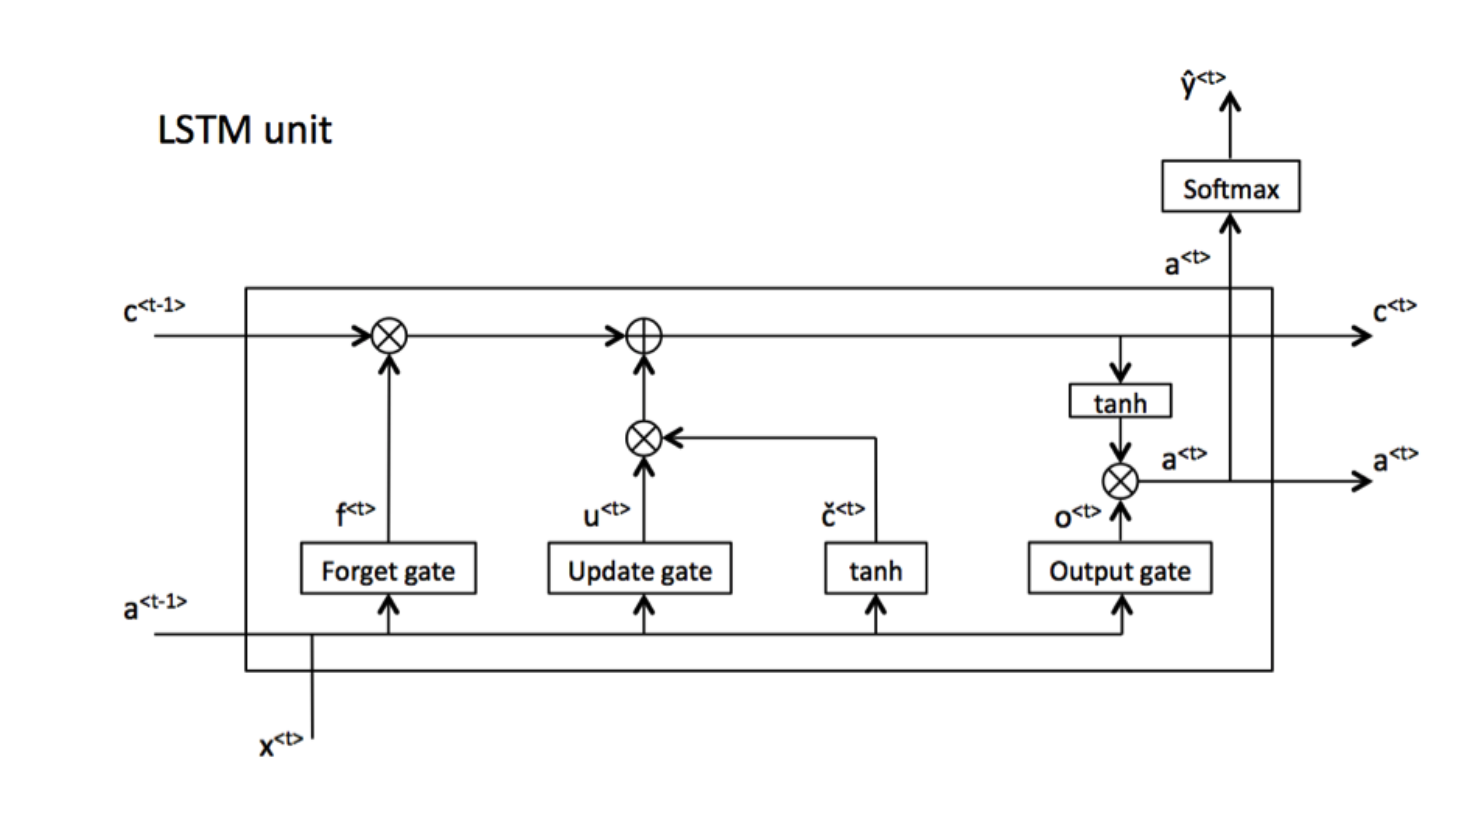
\includegraphics[height=0.25\paperheight]{Figures/LSTM_cell.png}
    \caption[LSTM Unit]{LSTM unit\cite{cavaioni_deeplearning_2018}}
    \label{fig:LSTM cell}
\end{figure}

LSTMs differ from GRUs in the candidate value for the memory cell. Instead of \(c^{<t-1>}\), \(a^<t-1>\) is used.
\[\Tilde{c}^{<t>}=tanh(W_c[\Gamma_r*a^{<t-1>},x^{<t>}]+b_c)\]
Another difference is that, instead of having only 1 update gate, \(\Gamma_u\), there are 2 gates - one for update, and another to forget, \(\Gamma_f\):
\[\Gamma_f = \sigma(W_f[c^{<t-1>},x^{<t>}]+b_f)\]
And another output gate \(\Gamma_o\), calculated as:
\[\Gamma_o = \sigma(W_o[c^{<t-1>},x^{<t>}]+b_o)\]
The new value in the memory cell is calculated using the gates defined above as:
 \[c^{<t>}=\Gamma_u*\Tilde{c}^{<t>} + \Gamma_f*{c}^{<t-1>} \]
 \[a^{<t>}=\Gamma_o*c^{<t>}\]

As LSTMs have many more parameters to be computed, networks with GRUs run faster than LSTMs. As pointed in \cite{chung_empirical_2014}, GRUs and LSTMs perform equally well, and it has not been proved that any one is superior. Hence in this work, we opt for a GRU unit,as it provides almost the same.

Given that RNNs are more appropriate for sequence data, and the problem we are trying to solve is a sequence of pedestrian positions, we will employ RNNs for pedestrian trajectory estimation. As GRUs and LSTMs are equally popular, and no unit has been proved to be superior compared to the other, a simple GRU unit will be used in this work.